\chapter{Preliminaries}\label{chap:preliminaries} 

In this chapter, we establish the foundational topological and geometric machinery required to prove our main detection result, Theorem \ref{thm:main_detection}.

To achieve this, we must translate a problem in three-dimensional topology into one of surface dynamics. Because the knot $T_{2,3} \# T_{2,3}$ is fibered, any knot sharing its knot Floer homological profile must also be fibered. This shifts the focus of our proof from the geometry of the knot to the mapping class group of its fiber surface. Consequently, our argument relies on weaving together the algebraic constraints of Heegaard Floer homology with the dynamical rigidity of surface homeomorphisms.

We structure this background material as follows. In Section \ref{sec:notation}, we fix the notational conventions used throughout the dissertation. In Section \ref{sec:fibered-hfk}, we review the basics of fibered knots and knot Floer homology, highlighting the pivotal theorems of Ozsv\'{a}th--Szab\'{o} and Ni which demonstrate that $\widehat{HFK}$ detects the Seifert genus and fiberedness of a knot. We then introduce the Nielsen-Thurston classification of surface mapping classes and its three-dimensional analogue, Thurston's geometric classification of knots.

In Section \ref{sec:pA}, we delve into the geometry of pseudo-Anosov mapping classes, which correspond precisely to hyperbolic knots. We detail their invariant singular foliations and characterize their twisting behavior near the boundary via the fractional Dehn twist coefficient. In Section \ref{section:fibered hyperblic}, we restrict our focus to hyperbolic fibered knots sharing the knot Floer homological profile of $T_{2,3} \# T_{2,3}$, utilizing recent work in Heegaard Floer homology and contact geometry to severely bound the fixed points and boundary prongs of their monodromies.

Finally, in Section \ref{section:Birman-Hilden}, we invoke the Birman-Hilden correspondence. This machinery allows us to project highly constrained, symmetric monodromies on the genus-two surface down to the punctured sphere and disk. This descent directly sets the stage for the combinatorial enumeration of pseudo-Anosov strata, which we carry out at the conclusion of the chapter.

\section{Notation and Conventions}\label{sec:notation}

Throughout this dissertation we adopt the following conventions; later chapters refer back to this section.

\paragraph{Surfaces.} We denote by $\Sigma_g^b$ the compact, oriented surface of genus $g$ with $b \ge 0$ boundary components and no marked points. When marked points are present, we write $\Sigma_{g,n}^b$ for the surface of genus $g$ with $b$ boundary components and $n$ marked points in its interior. When $b=0$, the marked-point notation reduces to $\Sigma_{g,n}$. The $n$-marked closed disk is denoted $D_n$, and we identify $D_n$ throughout with the closed unit disk in $\mathbb{C}$ together with $n$ designated marked points. The $n$-marked sphere is denoted $S^2_{0,n}$, or simply $S^2_n$ when no confusion arises.

\paragraph{Mapping classes.} The mapping class group of a surface $\Sigma$ is denoted $\mathrm{Mod}(\Sigma)$, and consists of isotopy classes of orientation-preserving homeomorphisms fixing $\partial \Sigma$ pointwise and preserving the set of marked points. The mapping class of a homeomorphism $f$ is denoted $[f]$. We use letters such as $h$, $\hat h$, $b$, $\beta$, $\Phi$ for mapping classes, and the corresponding $\phi$-decorated symbols ($\phi_h$, $\hat{\phi}_h$, $\phi_b$, $\phi_\beta$, $\phi_\Phi$) for chosen geometric (typically pseudo-Anosov) representatives.

\paragraph{The hyperelliptic involution.} The hyperelliptic involution of $\Sigma_2^0$ is denoted $\iota$ throughout this dissertation. We reserve the symbol $\tau$ for train tracks (Chapters \ref{chap:folding_automata}--\ref{chap:stratatraintrackanalysis}); these two notational roles are kept strictly disjoint.

\paragraph{Field of coefficients.} Unless explicitly stated otherwise, all knot Floer homology groups in this dissertation are taken with coefficients in the field $\mathbb{F} := \mathbb{Z}/2\mathbb{Z}$. The detection results of Ghiggini \sidecite{Ghi08}, Ni \sidecite{Ni07}, and Juh\'{a}sz \sidecite{Juh08} were originally established over $\mathbb{Q}$ but extend to $\mathbb{F}$; see the discussion in \cite[\S 2]{baldwin2025khovanov} for the relevant coefficient-ring considerations.

\paragraph{The Birman-Hilden correspondence data.} A central object in this dissertation is the ordered tuple
\[
(h, \phi_h, \hat{h}, \hat{\phi}_h, b, \phi_b, \beta, \phi_\beta, \Phi, \phi_\Phi),
\]
which we shall refer to as the \emph{Birman-Hilden correspondence data} associated to a hyperbolic fibered knot $K$ satisfying $\widehat{HFK}(K) \cong \widehat{HFK}(T_{2,3}\# T_{2,3})$. The construction and properties of this tuple are developed in detail in Section \ref{section:Birman-Hilden}.

\section{Fibered Knots and Knot Floer Homology}
\label{sec:fibered-hfk}

Let $K \subset S^3$ be a knot and let $N(K)$ denote its open tubular neighborhood. We say that $K$ is \textbf{fibered} if the knot exterior $E(K) = S^3 \setminus N(K)$ admits the structure of a fiber bundle over the circle $S^1$. More precisely, there exists a smooth submersion
\[
\pi: E(K) \to S^1
\]
such that for every $\theta \in S^1$, the preimage
\[
\Sigma_\theta = \pi^{-1}(\theta)
\]
is a compact, orientable surface with boundary $\partial \Sigma_\theta = K$. The fiber $\Sigma_\theta \cong \Sigma_g^1$ (where $g$ is the Seifert genus of $K$) is a minimal genus Seifert surface for $K$, and the fibration is entirely determined by the monodromy diffeomorphism
\[
h: \Sigma_g^1 \to \Sigma_g^1,
\]
which is defined up to isotopy fixing the boundary pointwise.

The knot exterior is thus homeomorphic to the mapping torus
\[
M_h = (\Sigma_g^1 \times [0,1]) / \sim,
\]
where $(x, 1) \sim (h(x), 0)$ for $x \in \Sigma_g^1$ and $(x, s) \sim (x, t)$ for $x \in \partial \Sigma_g^1$ and all $s,t \in [0,1]$.

\subsection*{Knot Floer Homology}
\textbf{Knot Floer homology}, introduced by Ozsv\'ath and Szab\'o \sidecite{OS04Knot}, and independently by Rasmussen \sidecite{Ras03}, provides a powerful knot invariant for distinguishing topological properties of $K$, including its genus and fiberedness. There are several flavors of knot Floer homology; however, in this thesis, we shall exclusively utilize the ``hat'' version with coefficients in the field $\mathbb{F} = \mathbb{Z}/2\mathbb{Z}$, denoted $\widehat{HFK}(K)$. This invariant is a bigraded vector space over $\mathbb{F}$:
\begin{equation}
    \widehat{HFK}(K) = \bigoplus_{M, A} \widehat{HFK}_M(K, A),
\end{equation}
where $M$ denotes the \textbf{Maslov grading} and $A$ denotes the \textbf{Alexander grading}. The Euler characteristic of this homology theory recovers the classical Alexander polynomial $\Delta_K(t)$:
\begin{equation}
    \Delta_K(t) = \sum_{M, A} (-1)^M \dim_{\mathbb{F}} \big( \widehat{HFK}_M(K, A) \big) t^A.
\end{equation}

A seminal result of Ozsv\'ath and Szab\'o establishes that knot Floer homology detects the Seifert genus of the knot, denoted $g(K)$. Specifically, the width of the homology in the Alexander grading is completely determined by the genus:
\begin{equation}\label{eq:ozvath-szabo genus top grading}
    g(K) = \max \{ A \mid \widehat{HFK}(K, A) \neq 0 \}.
\end{equation}

Of central importance to this work is the ability of knot Floer homology to detect fibered knots. While it is well-known that the Alexander polynomial provides a necessary condition for fiberedness---namely, that $\Delta_K(t)$ must be monic---it is not sufficient (for example, any non-trivial untwisted Whitehead double possesses a trivial Alexander polynomial but is never fibered). On the other hand, knot Floer homology provides a necessary and sufficient condition. This detection result was established by Ghiggini \sidecite{Ghi08} for genus-one knots and by Ni \sidecite{Ni07} for arbitrary genus.

\begin{theorem}[Ni \cite{Ni07}]
    \label{theorem:ni-fibered}
    A knot $K \subset S^3$ is fibered if and only if
    \begin{equation}
        \dim_{\mathbb{F}} \widehat{HFK}(K, g(K)) = 1.
    \end{equation}
\end{theorem}

In other words, $K$ is fibered if and only if the knot Floer homology in the top Alexander grading is one-dimensional. Consequently, for a fibered knot, the top-graded component is supported in a single Maslov grading. This theorem reduces the deeply topological question of the existence of a fibration to an algebraic computation of the rank of $\widehat{HFK}(K)$.

\subsection*{The Monodromy and the Nielsen-Thurston Classification}
As a consequence of Theorem \ref{theorem:ni-fibered}, if a hypothetical knot $K$ satisfies the hypothesis of Theorem \ref{thm:main_detection}:
\[
\widehat{HFK}(K) \cong \widehat{HFK}(T_{2,3} \# T_{2,3})
\]
as bigraded vector spaces, then it is immediate that $K$ is a fibered knot of genus two. The bulk of the work required to prove Theorem \ref{thm:main_detection} involves the rigorous study of the monodromy $h \colon \Sigma_2^1 \to \Sigma_2^1$ of such a fibered knot.

A simple closed curve on $\Sigma_{g,n}^b$ is \textbf{essential} if it does not bound a disk, a once-punctured disk, or an annulus cobounding a boundary component of $\Sigma_{g,n}^b$. A \textbf{multicurve} is a finite collection of disjoint, pairwise non-isotopic, essential simple closed curves.

The Nielsen-Thurston Classification Theorem provides a fundamental structural trichotomy for elements of the mapping class group.

% [NOTE ON EULER CHARACTERISTIC]
% The condition \chi < 0 is strictly necessary to form a true trichotomy. 
% It excludes the unmarked sphere (which has a trivial/degenerate mapping 
% class group) and the torus (which admits Anosov maps with perfectly smooth 
% foliations and no singular prongs, violating the pseudo-Anosov definition). 
% 
% Importantly, this theorem perfectly covers our later use of the marked disk. 
% An n-marked disk D_n has Euler characteristic \chi(D_n) = 1 - n. Since we 
% use n = 5 and n = 6 marked points for our braids, our disks strictly 
% satisfy \chi < 0.
\begin{theorem}[Nielsen-Thurston Classification \cite{Thurston1988}]\label{theorem:nielsen-thruston classification}
Let $\Sigma$ be a compact, orientable surface with negative Euler characteristic. Every mapping class $[h] \in \mathrm{Mod}(\Sigma)$ satisfies exactly one of the following mutually exclusive conditions:
\begin{itemize}
    \item \textbf{Periodic:} There exists an integer $m > 0$ such that $[h]^m = [\id]$. Equivalently, by the Nielsen Realization Theorem, $[h]$ contains a representative homeomorphism $f$ such that $f^m = \id$ pointwise.
    \item \textbf{Reducible:} The mapping class $[h]$ is not periodic, and there exists a multicurve $\Gamma = \{\gamma_1, \dots, \gamma_k\}$ on $\Sigma$ that is invariant under $[h]$. That is, $h(\Gamma)$ is isotopic to $\Gamma$.
    \item \textbf{Pseudo-Anosov:} The mapping class $[h]$ contains a unique geometric representative $\phi_h$ (up to conjugacy by isometries) that preserves a pair of transverse, measured singular foliations: the stable foliation $(\mathcal{F}_s, \mu_s)$ and the unstable foliation $(\mathcal{F}_u, \mu_u)$. Furthermore, there exists a real number $\lambda > 1$, called the \emph{dilatation}, such that $\phi_h(\mathcal{F}_s, \mu_s) = (\mathcal{F}_s, \lambda^{-1} \mu_s)$ and $\phi_h(\mathcal{F}_u, \mu_u) = (\mathcal{F}_u, \lambda \mu_u)$.
\end{itemize}
\end{theorem}

We will refer to the mapping class $[h]$ as periodic, reducible, or pseudo-Anosov according to the geometric type of its representative. More details on pseudo-Anosov maps will be provided in Section \ref{sec:pA}.

\subsection*{Thurston's Trichotomy for Knots}
The \emph{Thurston classification of knots} is the three-dimensional geometric realization of the Nielsen-Thurston classification of surface mapping classes. For a fibered knot $K \subset S^3$ with fiber $\Sigma_g^1$ and monodromy $h$, the knot exterior $E(K)$ is homeomorphic to the mapping torus $M_h$.

The dynamical properties of the mapping class $[h]$ directly dictate the three-dimensional topology and geometry of $M_h$. Thurston demonstrated that every knot $K \subset S^3$ falls into exactly one of three geometric categories, which perfectly mirror the two-dimensional classification:

\begin{theorem}[Thurston's Classification of Knots \cite{Thurston1982}] \label{theorem:thurston classification of knots}
    Every knot $K \subset S^3$ is exactly one of the following: a torus knot, a satellite knot, or a hyperbolic knot.
\end{theorem}

For fibered knots, this three-dimensional geometric trichotomy is in bijective correspondence with the two-dimensional dynamical trichotomy of the monodromy:
\begin{itemize}
    \item \textbf{Torus Knots (Periodic):} If $[h]$ is periodic, the mapping torus $M_h$ admits a Seifert fibered structure. In $S^3$, the only fibered knots with Seifert fibered complements are the torus knots $T_{p,q}$, which can be embedded on the surface of an unknotted torus.
    \item \textbf{Satellite Knots (Reducible):} If $[h]$ is reducible, the invariant multicurve $\Gamma \subset \Sigma_g^1$ sweeps out a finite union of incompressible, non-boundary-parallel tori $\Gamma \times S^1$ in the mapping torus $M_h$. The existence of such an essential torus in $E(K)$ is the exact definition of a satellite knot. We provide more details in Chapter \ref{chap:satellite}.
    \item \textbf{Hyperbolic Knots (Pseudo-Anosov):} If $[h]$ is pseudo-Anosov, the invariant measured foliations on $\Sigma_g^1$ can be suspended to construct a complete Riemannian metric of constant negative curvature on the interior of $M_h$. Thus, $S^3 \setminus K$ is a hyperbolic 3-manifold of finite volume.
\end{itemize}

The proof strategy for Theorem \ref{thm:main_detection} relies entirely on this geometric bridge. We will systematically assume the hypothetical knot $K$ belongs to each of Thurston's three geometric categories: torus, satellite, and hyperbolic. We will then eliminate all distinct knot candidates in each category. We note immediately that the torus knot case is entirely trivial; the Alexander polynomials of torus knots are completely classified, and none can possibly coincide with the observed polynomial $\Delta_K(t) = (t - 1 + t^{-1})^2$. Thus, the topological obstruction rests entirely on eliminating the satellite and hyperbolic cases.

\section{Pseudo-Anosov Maps}\label{sec:pA}
The case where $K$ is assumed to be a hyperbolic knot will be the most geometrically involved and will constitute the bulk of this thesis. As established by the trichotomy correspondence above:

\begin{theorem}[Thurston \cite{Thu98}] \label{theorem:Thurston hyperbolic iff pA}
    Let $K$ be a fibered knot with monodromy $h$. The knot complement $S^3 \setminus K$ admits a complete hyperbolic metric of finite volume if and only if $[h]$ is pseudo-Anosov. In other words, $K$ is hyperbolic if and only if $h$ is freely isotopic to a pseudo-Anosov map $\phi_h$.
\end{theorem}

Let $\phi \colon \Sigma_{g,n}^b \to \Sigma_{g,n}^b$ be a pseudo-Anosov homeomorphism permuting the marked points $\mathcal{P}$. The stable and unstable singular foliations $(\mathcal{F}_s, \mu_s)$ and $(\mathcal{F}_u, \mu_u)$ have singularities in the interior of $\Sigma_{g,n}^b$ that are required to be ``$k$-pronged saddles'' with $k \geq 3$. Each foliation must have at least one singularity on every boundary component. For marked points, the foliations are permitted to have 1-pronged singularities. Note that the singularities of $\mathcal{F}_s$ and $\mathcal{F}_u$ perfectly coincide and exhibit the identical number of prongs with respect to both foliations.

We illustrate the local models for these allowable singularities in Figure \ref{fig:pA_prong_types}. As depicted, non-marked interior singularities must exhibit three or more prongs, corresponding to the traditional saddle points of the invariant foliations. In contrast, marked points (or punctures) may host 1-pronged or 2-pronged configurations, as the foliation is permitted to terminate or pass smoothly through these designated points. Similarly, a boundary component can support any integer number of prongs $k \ge 1$, with the invariant leaves terminating at the boundary curve.

\begin{figure}[h]
    \centering
    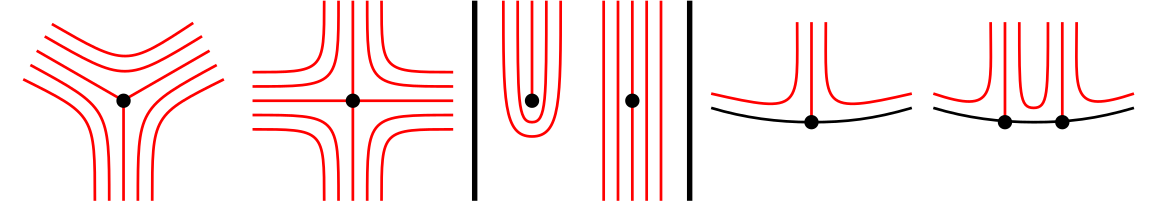
\includegraphics[width=\linewidth]{figures/pA_prong_types.png}
    \caption[Allowable singularities in pseudo-Anosov invariant foliations]{The allowable singularities in the invariant foliations of a pseudo-Anosov map. Non-marked interior singularities must have at least 3 prongs. Left: a 3-pronged and a 4-pronged singularity. Center: a 1-pronged and a 2-pronged singularity at a marked point. Right: a 1-pronged and a 2-pronged boundary component. Image courtesy of Braeden Reinoso \cite{reinoso2024pseudo}.}
    \label{fig:pA_prong_types}
\end{figure}

Locally, one should view a pseudo-Anosov map $\phi$ as stretching the surface in the direction of $\mathcal{F}_u$ and shrinking it in the transverse direction described by $\mathcal{F}_s$. Because the invariant foliations are set-wise preserved by $\phi$, the map must always permute singular points that possess the same number of prongs.

\subsection*{Singularity Types}
Following the convention of Farber, Reinoso, and Wang \sidecite{farber2024fixed}, we utilize the following notation. The \emph{singularity type} of a pseudo-Anosov map $\phi$ is the tuple recording the number of prongs at each singularity:
\[
(b_1, \dots, b_r; \, m_1, \dots, m_n; \, k_1, \dots, k_s)
\]
where the $i$th boundary component of $\phi$ has $b_i$ prongs; the $i$th marked point has $m_i$ prongs; and the $i$th non-marked interior singularity has $k_i$ prongs. We use $\emptyset$ if there are no singularities of a certain type, and exponents to denote multiple singularities possessing the same number of prongs.

For example, the tuple $(2; 1^6; 3^2)$ indicates that the foliations have a 2-pronged singularity at the unique boundary component; six 1-pronged singularities at marked points; and two 3-pronged non-marked interior singularities. If the surface has an empty boundary, we suppress the $b_i$ entries entirely. For instance, the stratum $(1^6; 3^2)$ on the sphere $S^2$ indicates six 1-pronged singularities at marked points and two 3-pronged interior singularities.

\subsection{Fractional Dehn Twist Coefficient}\label{subsection:FDTC}
The \textbf{fractional Dehn twist coefficient}, denoted $c(h)$, is a rational number that quantifies the amount of twisting of the monodromy near the boundary $\partial \Sigma_g^1$.

\begin{definition}
\label{def:fdtc}
Let $h \in \mathrm{Mod}(\Sigma_g^1)$ be a mapping class with pseudo-Anosov representative $\phi_h$. The fractional Dehn twist coefficient $c(h)$ is defined as
\[
c(h) = n + \frac{m}{k},
\]
where:
\begin{itemize}
    \item $n \in \mathbb{Z}$ is the number of full Dehn twists $h$ performs near $\partial \Sigma_g^1$ relative to $\phi_h$.
    \item $k \geq 1$ is the number of singular points (prongs) of the invariant foliations on $\partial \Sigma_g^1$.
    \item The geometric map $\phi_h$ permutes these $k$ singular points on the boundary by a fractional rotation of $m$ steps in the counter-clockwise direction.
\end{itemize}
\end{definition}

\begin{theorem}[{\cite[Theorem~2.1.4]{reinoso2024pseudo}}]
   Let $\Sigma$ be a compact surface, possibly with marked points, and let $h \in \mathrm{Mod}(\Sigma)$ be a pseudo-Anosov mapping class. Then:
   \begin{enumerate}
       \item $c(h)$ is preserved under conjugation within $\mathrm{Mod}(\Sigma)$.
       \item $c(\id) = 0$ and $c(T_{\partial \Sigma}^n \circ h) = n + c(h)$, where $T_{\partial \Sigma}$ is a positive boundary Dehn twist.
   \end{enumerate}
\end{theorem}
Given a fibered knot $K$, we define $c(K) \coloneqq c(h)$ where $(\Sigma_g^1, h)$ is the open book associated to $K$. The conjugation invariance ensures this is a well-defined knot invariant.

\section{Fibered Hyperbolic Knots}\label{section:fibered hyperblic}
To prove our main result, we must rule out the existence of a distinct hyperbolic knot $K$ whose knot Floer homology coincides with $T_{2,3} \# T_{2,3}$. Let $K$ be a hyperbolic knot such that
\[
\widehat{HFK}(K) \cong \widehat{HFK}(T_{2,3} \# T_{2,3})
\]
as bigraded vector spaces. By the discussion in Section \ref{sec:fibered-hfk}, $K$ is immediately known to be fibered and of genus two. Let
\[
h \colon \Sigma_2^1 \to \Sigma_2^1
\]
denote the monodromy of $K$. By Theorem \ref{theorem:Thurston hyperbolic iff pA}, $[h]$ is pseudo-Anosov. Let $\phi_h$ be its geometric representative.

\subsection*{Fixed Points}
The work of Ghiggini-Spano, and independently of Ni, establishes that the next-to-top Alexander grading of $K$ severely bounds the number of fixed points of $\phi_h$:

\begin{theorem}[{\cite[Theorem 1.2]{ghiggini2022heegaard}}, \cite{Ni2022}]
    Let $Y$ be a closed, oriented 3-manifold, and $K \subset Y$ be a hyperbolic fibered knot with fiber $\Sigma$ and monodromy $h$. If
    \[
    \dim_{\mathbb{F}} \widehat{HFK}(Y, K, [\Sigma], g(\Sigma) - 1) = r,
    \]
    then $h$ is freely isotopic to a pseudo-Anosov map $\phi_h$ with at most $r - 1$ fixed points.
\end{theorem}

In our case, the next-to-top Alexander grading is of rank two:
\[
    \dim_{\mathbb{F}} \widehat{HFK}(S^3, K, [\Sigma_2^1], 1)= \dim_{\mathbb{F}} \widehat{HFK}(S^3, T_{2,3} \# T_{2,3}, [\Sigma_2^1], 1) = 2.
\]
Hence $\phi_h$ has at most one fixed point. The work of Farber, Reinoso, and Wang \sidecite{farber2024fixed} eliminates the possibility that there are no fixed points:

\begin{lemma}[Farber--Reinoso--Wang \cite{farber2024fixed}]\label{lemma:original monodromy has one fixed point}
    Let $K$ be a hyperbolic, fibered knot with monodromy $h$, and suppose $\widehat{HFK}(K) \cong \widehat{HFK}(T_{2,3} \# T_{2,3})$. Then $\phi_h$ has exactly one fixed point in the interior of $\Sigma_2^1$.
\end{lemma}
\begin{proof}
    Farber, Reinoso, and Wang \sidecite{farber2024fixed} classified all pseudo-Anosov monodromies on the genus-two surface with one boundary component and no interior fixed points. They showed that the only such monodromy arising from a fibered knot in $S^3$ belongs to the cinquefoil $T(2,5)$. The cinquefoil has a completely different knot Floer homology from $T_{2,3} \# T_{2,3}$, which is immediately deduced from the fact that $\Delta_{T(2,5)}(t) = t^2 - t + 1 - t^{-1} + t^{-2}$.
\end{proof}

\subsection*{Capping Off}\label{subsec:capping_off}
The work of Baldwin-Hu-Sivek \sidecite{baldwin2025khovanov} demonstrates that when there is more than one prong on the boundary of $\Sigma_2^1$, the geometric map $\phi_h$ extends naturally to a ``capped-off'' pseudo-Anosov map
\[
\hat{\phi}_h \colon \Sigma_2^0 \to \Sigma_2^0
\]
on the closed genus-two surface $\Sigma_2^0$, obtained by capping $\partial \Sigma_2^1$ with a disk. The invariant foliations extend to stable and unstable foliations $\hat{\mathcal{F}}^s$ and $\hat{\mathcal{F}}^u$, where the $n$-prongs on $\partial \Sigma_2^1$ meet at a newly formed singularity $p$ in the capping disk. Note that $p$ is inherently a fixed point of $\hat{\phi}_h$.

We now show that $\phi_h$ must have more than one prong on the boundary $\partial \Sigma_2^1$, allowing for such a capping off and extension of the foliations. The following argument follows Baldwin-Hu-Sivek closely, but with more details:

\paragraph{Thinness and the $\tau$ invariant} The composite knot $T_{2,3} \# T_{2,3}$ is an alternating knot and is therefore \textbf{knot Floer thin}, as established by Ozsv\'{a}th and Szab\'{o} \sidecite{ozsvath2003heegaard}. Its homology is supported entirely on the diagonal $\delta = A - M = \sigma/2$. Since $\widehat{HFK}(K) \cong \widehat{HFK}(T_{2,3} \# T_{2,3})$, $K$ is also thin. For thin knots, the spectral sequence from $\widehat{HFK}$ to $\widehat{HF}(S^3)$ collapses immediately, meaning the $\tau$ invariant is determined entirely by the grading support. Since $\tau(T_{2,3} \# T_{2,3}) = 2$, we deduce that
\[
\tau(K) = g(K) = 2.
\]

\paragraph{Strong quasipositivity} By the work of Hedden \sidecite{Hedden2010}, a fibered knot $K$ satisfies $\tau(K) = g(K)$ if and only if $K$ is strongly quasipositive. In terms of contact topology, this implies the open book decomposition of $S^3$ with binding $K$ supports the standard tight contact structure $\xi_{std}$.

\paragraph{Right-veering monodromy} Let $(\Sigma_2^1, h)$ be the abstract open book associated to $K$. By Honda, Kazez, and Matić \sidecite{honda2007right}, the contact structure supported by $(\Sigma_2^1, h)$ is tight if and only if the monodromy $h$ is right-veering. This implies the fractional Dehn twist coefficient satisfies $c(h) \ge 0$. Since $K$ is hyperbolic, $h$ is pseudo-Anosov and thus irreducible. Honda, Kazez, and Matić establish that a right-veering diffeomorphism with $c(h)=0$ must be reducible. We therefore conclude $c(h) > 0$.

\paragraph{Prongs of the invariant foliation} Recall that $c(h) = n + \frac{m}{k}$, where $k$ is the number of prongs on the boundary. A result of Hedden-Mark (Proposition \ref{prop:hedden_mark_remark} below) implies that for fibered hyperbolic knots, $\abs{c(h)} < 1$.

\begin{prop}[{\cite[Remark 2.7]{hedden2018floer}}]\label{prop:hedden_mark_remark}
    If $K \subset S^3$ is a fibered hyperbolic knot with monodromy $h$, then $\abs{c(h)} < 1$.
\end{prop}

Since $0 < c(h) < 1$, the coefficient is strictly non-integer, meaning the singularity at the boundary cannot be 1-pronged. Therefore, the invariant foliation must possess $k \ge 2$ prongs on the boundary.

\begin{remark}
    Remark 2.7 of Hedden-Mark states the result of Proposition \ref{prop:hedden_mark_remark} for an arbitrary fibered knot in an $L$-space without assuming hyperbolicity. They cite a result of Honda-Kazez-Mati\'{c} \sidecite{honda2007right} that when $|c(h)| \geq 1$, the $L$-space admits a taut foliation. However, this cited result strictly requires the assumption of hyperbolicity.
\end{remark}



\section{The Birman-Hilden Correspondence and Monodromy Descent} \label{section:Birman-Hilden}

In this section, we establish the geometric machinery required to relate the monodromy of the knot $K$ to a braid on the sphere, and subsequently to a braid on the disk. This relationship relies on the geometric symmetries of the closed genus-two surface, which in accordance with the discussion in Section \ref{subsec:capping_off}, should be thought of as arising from capping-off the monodromy of the hyperbolic knot $K$.

Recall that for the closed genus-two surface $\Sigma_2^0$, the mapping class group $\mathrm{Mod}(\Sigma_2^0)$ contains a distinguished element $[\iota]$, known as the \textbf{hyperelliptic involution}. Algebraically, $[\iota]$ is the unique non-trivial element in the center of $\mathrm{Mod}(\Sigma_2^0)$. Consequently, for any mapping class $[\hat{\phi}_h] \in \mathrm{Mod}(\Sigma_2^0)$, we have the commutation relation:
\begin{equation}\label{equation:symmetric hyperelliptic involution}
    [\hat{\phi}_h][\iota] = [\iota][\hat{\phi}_h].
\end{equation}
We call a geometric representative $\iota \colon \Sigma_2^0 \to \Sigma_2^0$ a hyperelliptic involution if it belongs to the class $[\iota]$.

The geometric utility of this involution is captured by the Birman-Hilden correspondence. Broadly speaking, this classical correspondence establishes an algebraic relationship between the subgroup of mapping classes that commute with a branched covering involution (the \textit{symmetric} mapping class group) and the mapping class group of the quotient surface marked by the branch data.

For the closed genus-two surface $\Sigma_2^0$, the hyperelliptic involution $[\iota]$ generates the center of $\mathrm{Mod}(\Sigma_2^0)$. Because every mapping class commutes with the center, \textit{every} mapping class on $\Sigma_2^0$ is symmetric. Consequently, the Birman-Hilden correspondence implies that $\mathrm{Mod}(\Sigma_2^0) / \langle [\iota] \rangle$ is isomorphic to $\mathrm{Mod}(S^2_{0,6})$, the mapping class group of the sphere with six marked points.

This algebraic isomorphism has profound geometric implications for surface dynamics. It guarantees that any pseudo-Anosov mapping class on $\Sigma_2^0$ can be projected down to a well-defined pseudo-Anosov map on the marked sphere. For our purposes, this descent is made precise by the following lemma of Baldwin, Hu, and Sivek:

\begin{lemma}[{\cite[Lemma~3.7]{baldwin2025khovanov}}]\label{lemma:Baldwinliftpseudoanosov}
    Let $\hat{h} \in \mathrm{Mod}(\Sigma_2^0)$ be a pseudo-Anosov mapping class with geometric representative $\hat{\phi}_h \colon \Sigma_2^0 \to \Sigma_2^0$. Then there exists a branched double covering
    \[
    \pi \colon \Sigma_2^0 \to S^2,
    \]
    branched along six points $q_1, \dots, q_6 \in S^2$, such that $\hat{\phi}_h$ is a lift of a pseudo-Anosov map
    \[
    \phi_b \colon (S^2, q_1, \dots, q_6) \to (S^2, q_1, \dots, q_6),
    \]
    representing a class $b \in \mathrm{Mod}(S^2_{0,6})$. Furthermore, the invariant foliations of $\hat{\phi}_h$ are lifts of those of $\phi_b$.
\end{lemma}

In the proof of Lemma \ref{lemma:Baldwinliftpseudoanosov}, it is shown that the double covering $\pi$ is the quotient map under the action of a hyperelliptic involution $\iota$ that commutes strictly (``on the nose'') with $\hat{\phi}_h$:
\[
\hat{\phi}_h \circ \iota = \iota \circ \hat{\phi}_h.
\]
The fixed points of the involution $\iota$ are exactly the pre-images of the branch points. Denoting these pre-images by $p_i = \pi^{-1}(q_i)$, we have $\mathrm{Fix}(\iota) = \{p_1, \dots , p_6\}$. These are called the \textbf{Weierstrass points} of $\Sigma_2^0$.

\subsection{Fixed Point Dynamics of the Capped Monodromy}

Recall that our hypothetical knot $K$ is fibered of genus two. Let $h \in \mathrm{Mod}(\Sigma_2^1)$ denote its monodromy class on the surface with one boundary component, and let $\phi_h \colon \Sigma_2^1 \to \Sigma_2^1$ be its unique pseudo-Anosov geometric representative.

By Lemma \ref{lemma:original monodromy has one fixed point}, we know that the original monodromy $\phi_h$ possesses exactly one fixed point in the interior of the surface, which we shall denote by $z$.

When extending $\phi_h$ to the closed surface $\Sigma_2^0$ by capping the boundary with a disk, we introduce exactly one new fixed point, $p$ (the center of the capping disk). Thus, the capped-off pseudo-Anosov map $\hat{\phi}_h$ has exactly two fixed points, $\{z, p\}$. The geometric fate of these two points under the branched covering is entirely dictated by the hyperelliptic involution, as established in the following proposition.

\begin{prop}[Capping Off, \cite{baldwin2025khovanov}]\label{prop:capping off}
Let $K$ be a hyperbolic, genus-two knot with monodromy class $h$ and pseudo-Anosov representative $\phi_h$. Suppose $\widehat{HFK}(K) \cong \widehat{HFK}(T_{2,3} \# T_{2,3})$. The capped off monodromy $\hat{\phi}_h \colon \Sigma_2^0 \to \Sigma_2^0$ is a pseudo-Anosov homeomorphism with exactly two fixed points, and the hyperelliptic involution $\iota$ swaps these two fixed points.
\end{prop}

\begin{proof}
By Lemma \ref{lemma:original monodromy has one fixed point}, $\phi_h$ has exactly one interior fixed point on $\Sigma_2^1$, which we denote $z$. Capping the boundary introduces one further fixed point $p$ at the center of the capping disk, so $\mathrm{Fix}(\hat{\phi}_h) = \{z, p\}$.

Since $\iota$ and $\hat{\phi}_h$ commute, $\iota$ preserves the fixed point set of $\hat{\phi}_h$. Thus, $\iota$ must either fix both $z$ and $p$ pointwise, or swap them.

Suppose, for the sake of contradiction, that $\iota(z) = z$ and $\iota(p) = p$. Then $z$ and $p$ are Weierstrass points and descend to branch points on $S^2$, say $\pi(z) = q_5$ and $\pi(p) = q_6$.

Consider $\Sigma_2^0$ punctured at $p$. The restriction of $\pi$ gives a double branched cover $\pi' \colon \Sigma_2^0 \setminus \{p\} \to S^2\setminus \{q_6\}$. Viewing these as the interiors of $\Sigma_2^1$ and $D^2$, the map $\hat{\phi}_h$ restricts to the original monodromy $h$ on $\Sigma_2^1$. It follows that $h$ is isotopic to the lift of a 5-braid mapping class
\[
\beta \colon (D_5, q_1,\dots,q_5) \to (D_5, q_1,\dots,q_5).
\]
Under our assumption, $z$ descends to the branch point $q_5$, forcing $q_5$ to be a fixed point of $\beta$. The associated permutation $\sigma_{\beta} \in S_5$ must fix the index 5. Consequently, the fifth strand of the braid forms a distinct link component $L_1$ of the closure $\hat{\beta}$, while the remaining strands form at least one other component. Thus, the closure $B = \hat{\beta}$ is a link with $\mu(B) \ge 2$ components.

The braid $\beta$ specifies an open book decomposition of $S^3$ whose branch set is $B$. The covering map $\pi'$ extends to a branched double covering between the manifolds $M_h \to M_\beta$. Since $K$ is a knot in $S^3$, we have $M_h \cong \Sigma(S^3,B) \cong S^3$. However, $b_1(\Sigma(S^3, B)) \ge \mu(B) - 1 \ge 1$, which implies $M_h$ cannot be $S^3$. This is a contradiction.

Therefore, the involution $\iota$ cannot fix $z$ and $p$. It must swap them: $\iota(z) = p$ and $\iota(p) = z$.
\end{proof}

\subsection{The Induced Map on the Disk}

As a consequence of Proposition \ref{prop:capping off}, $z$ and $p$ descend to a single point $r \in S^2$ that is \emph{not} a branch point. Since $z$ and $p$ are fixed by $\hat{\phi}_h$, $r$ is a fixed point of the spherical pseudo-Anosov map $\phi_b$.

We perform a real blow-up at $r$. We identify the punctured sphere $S^2 \setminus \{r\}$ with the interior of the standard unit disk, $\mathrm{int}(D^2)$. The six branch points $Q = \{q_1, \dots, q_6\}$ correspond to marked points. The map $\phi_b|_{S^2 \setminus \{r\}}$ extends continuously to a pseudo-Anosov homeomorphism $\phi_\beta \colon D^2 \to D^2$ of the closed disk. We define $\beta$ to be the associated mapping class.

\subsection{The Fixed-Point-Free Lift $\phi_\Phi$}

We now lift the disk homeomorphism $\phi_\beta$ back to the genus-two surface, with two boundary components. Let $\Sigma_2^2$ denote the compact surface obtained from $\Sigma_2^0$ by performing a real blow-up at the points $z$ and $p$. Topologically, $\Sigma_2^2$ is a genus-two surface with two boundary components.

The branched covering $\pi$ restricts to a map $\pi' \colon \Sigma_2^2 \to D^2$. The map $\phi_\beta$ lifts under $\pi'$ to a homeomorphism
\[
\phi_\Phi \colon \Sigma_2^2 \to \Sigma_2^2.
\]
By construction, $\phi_\Phi$ coincides with the restriction of the capped-off monodromy $\hat{\phi}_h$ to the complement of its fixed points. Since the fixed set of $\hat{\phi}_h$ was exactly $\{z, p\}$ (which now form the boundaries), $\phi_\Phi$ has no fixed points in the interior of the surface. Thus, $\phi_\Phi$ serves as a fixed-point-free pseudo-Anosov representative on $\Sigma_2^2$.

\subsection{General Framework: Braids and Prongs}

The constructions above yield what we shall term the \emph{Birman-Hilden correspondence data}, an ordered tuple completely capturing the algebraic and geometric descent of the monodromy:
\[
(h, \phi_h, \hat{h}, \hat{\phi}_h, b, \phi_b, \beta, \phi_\beta, \Phi, \phi_\Phi)
\]

\begin{enumerate}
    \item $h \in \mathrm{Mod}(\Sigma_2^1)$ is the original monodromy class of the hyperbolic knot $K$.
    \item $\phi_h \colon \Sigma_2^1 \to \Sigma_2^1$ is the unique pseudo-Anosov representative of $h$. It has exactly one interior fixed point, $z$.
    \item $\hat{h} \in \mathrm{Mod}(\Sigma_2^0)$ is the capped-off mapping class on the closed surface.
    \item $\hat{\phi}_h \colon \Sigma_2^0 \to \Sigma_2^0$ is the pseudo-Anosov representative of $\hat{h}$. It possesses exactly two fixed points: the inherited point $z$, and the new capping center $p$.
    \item $b \in \mathrm{Mod}(S^2_{0,6})$ is the spherical mapping class obtained by descending $\hat{h}$ via the hyperelliptic involution.
    \item $\phi_b \colon S^2 \to S^2$ is the pseudo-Anosov representative of $b$. It permutes the six branch points and has exactly one non-marked fixed point $r$, which is the geometric descent of $z$ and $p$.
    \item $\beta \in \mathrm{Mod}(D_6)$ is the 6-braid mapping class on the disk, obtained by performing a real blow-up of $S^2$ at the fixed point $r$.
    \item $\phi_\beta \colon D^2 \to D^2$ is the pseudo-Anosov representative of $\beta$, fixing the boundary $\partial D^2$ set-wise and permuting the six marked points.
    \item $\Phi \in \mathrm{Mod}(\Sigma_2^2)$ is the mapping class obtained by lifting $\beta$ back to the genus-two surface with two boundary components (the real blow-up of $z$ and $p$).
    \item $\phi_\Phi \colon \Sigma_2^2 \to \Sigma_2^2$ is the pseudo-Anosov representative of $\Phi$. It is strictly fixed-point-free in its interior.
\end{enumerate}

\begin{figure}[H]
    \centering
    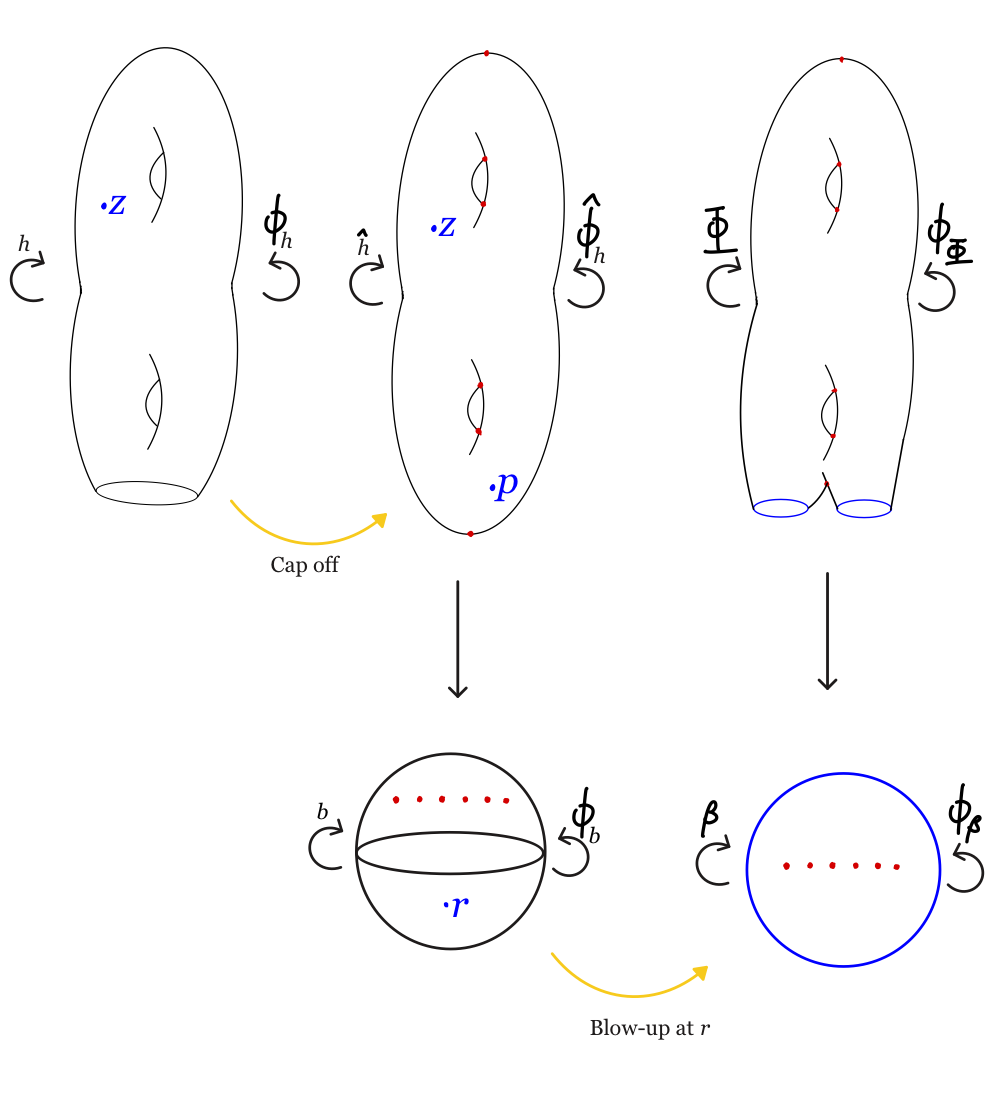
\includegraphics[width=\linewidth]{figures/BH.png}
    \caption{The Birman-Hilden Correspondence data.}
    \label{fig:birman_hilden_data}
\end{figure}

When $h$ is pseudo-Anosov, its invariant foliations descend to the disk $D^2$. To understand the geometric relationship between the singularities of $\phi_\beta$ and $\phi_h$, we must examine the local behavior of the branched covering map $\pi$. As detailed by Reinoso \cite[Section 2.2]{reinoso2024pseudo}, away from the branch locus, $\pi$ is a local diffeomorphism; pulling back a singular foliation through a local diffeomorphism preserves the number of prongs but duplicates the singularity in the cover. Conversely, at the branch points, the covering map behaves locally like the complex map $w = z^2$. Pulling back a measured foliation through this purely quadratic map doubles the cone angle, effectively doubling the number of prongs.

Consequently, the geometric singularities relate via the following rigid dictionary:
\begin{itemize}
    \item A $k$-pronged singularity of $\phi_\beta$ at a marked point (the branch locus) lifts to a single $2k$-pronged singularity of $\hat{\phi}_h$ because the covering map branches over these points, doubling the cone angle.
    \item A $k$-pronged singularity of $\phi_\beta$ on the boundary $\partial D^2$ (the blown-up unbranched point $r$) lifts to two distinct $k$-pronged boundaries $\partial_z$ and $\partial_p$ on $\Sigma_2^2$, which correspond to $k$-pronged singularities at $z$ and $p$ on $\Sigma_2^0$.
    \item A $k$-pronged singularity of $\phi_\beta$ in the interior of the disk (away from branch points) lifts to two distinct $k$-pronged singularities of $\hat{\phi}_h$, which are necessarily permuted by the hyperelliptic involution $\iota$.
\end{itemize}

\section{Strata}\label{sec:euler_poincare}
With this geometric dictionary established, we are now equipped to classify all possible Birman-Hilden correspondence data where $h$ is the monodromy of a hyperbolic knot $K$ satisfying $\widehat{HFK}(K) \cong \widehat{HFK}(T_{2,3} \# T_{2,3})$. We first enumerate all possible singularity structures (strata) that $\hat{\phi}_h$ can exhibit on $\Sigma_2^0$.

\begin{prop}[Euler-Poincar\'{e} Formula, {\cite[Proposition 11.4]{FarbMargalit2012}}]\label{prop:EulerPoincare}
    Let $\Sigma$ be a surface with a singular foliation. Let $P_s$ denote the number of prongs at a singular point $s$. Then
    \[
    2 \chi(\Sigma) = \sum_s (2 - P_s)
    \]
    where the sum is over all singular points.
\end{prop}
Applying this to the capped-off pseudo-Anosov $\hat{\phi}_h \colon \Sigma_2^0 \to \Sigma_2^0$, we obtain
\begin{equation}\label{equation:euler-poincare}
    -4 = \sum_s (2 - P_s).
\end{equation}

The possible sets of prongs $(P_s > 2)$ that satisfy this sum are:
\begin{itemize}
    \item \{3, 3, 3, 3\}
    \item \{3, 3, 4\}
    \item \{4, 4\}
    \item \{5, 3\}
    \item \{6\}
\end{itemize}

We can immediately eliminate the $\{5,3\}$ case. The map $\hat{\phi}_h$ must permute singularities with identical prong counts. Thus, it would fix the 5-pronged and 3-pronged singularities, forcing them to be exactly $z$ and $p$. However, by Proposition \ref{prop:capping off}, $\iota$ swaps $z$ and $p$, which implies they must have identical local geometry (the same number of prongs).

We can also eliminate $\{3,3,4\}$ and $\{6\}$. Since a pseudo-Anosov map must preserve singularity types, the unique 4-pronged or 6-pronged singularity in these sets would be forced to map to itself, constituting a third interior fixed point. This contradicts our established fact that $\mathrm{Fix}(\hat{\phi}_h)$ contains exactly two points.

Thus, the only valid sets of singularities are $\{3,3,3,3\}$ and $\{4,4\}$. Bearing in mind that $p$ and $z$ must have the exact same number of prongs (which could also be 2, meaning they are smooth points), the possible configurations are summarized in Table \ref{tab:betti_configurations}.

\begin{table}[ht]
    \centering
    \begin{tabular}{c c l}
        \toprule
        Prongs on $p$ & Prongs on $z$ & Prongs on other Singularities \\
        \midrule
        2 & 2 & \{4,4\} or \{3,3,3,3\}\\
        3 & 3 & \{3,3\} \\
        4 & 4 & $\emptyset$ \\
        \bottomrule
    \end{tabular}
    \caption{Possible singularity configurations satisfying the Euler-Poincar\'{e} formula.}
    \label{tab:betti_configurations}
\end{table}

We analyze each case to determine the precise strata on $\Sigma_2^0$, $S^2$, and $D^2$.

\subsection{Two prongs on $z$ and $p$}
If $z$ and $p$ are 2-pronged (smooth) points, the stratum $(4;4)$ is immediately eliminated since the remaining single 4-pronged singularity would be a fixed point.

For the stratum $(4,4;\emptyset)$, two marked points are 4-pronged singularities. $\iota$ fixes them, and $\hat{\phi}_h$ swaps them. This descends to $(2^2,1^4;2)$ on $S^2$, which corresponds to $(2;1^4,2^2; \emptyset)$ on $D^2$.

For $(\emptyset; 4,4)$, two unmarked points are 4-pronged. $\iota$ swaps them, and $\hat{\phi}_h$ swaps them. This descends to $(1^6;4)$ on $S^2$, corresponding to $(2;1^6;4)$ on $D^2$.

For the $\{3,3,3,3\}$ case, marked points cannot be odd-pronged, leaving only $(\emptyset; 3,3,3,3)$. The four 3-pronged unmarked points are permuted without fixed points. This descends to $(1^6;3^2)$ on $S^2$, corresponding to $(2;1^6;3^2)$ on $D^2$.

\begin{table}[ht]
    \centering
    \begin{tabular}{c c l}
        \toprule
        Stratum on $\Sigma_2^0$ & Stratum on $S^2$ & Stratum on $D^2$ \\
        \midrule
        $(4,4;\emptyset)$ & $(2^2,1^4;2)$ & $(2;1^4,2^2;\emptyset)$ \\
        $(\emptyset;4,4)$ & $(1^6;4)$ & $(2;1^6;4)$ \\
        $(\emptyset; 3,3,3,3)$ & $(1^6;3^2)$ & $(2;1^6;3^2)$\\
        \bottomrule
    \end{tabular}
    \caption{The strata with two prongs on $z$ and $p$.}
    \label{tab:strata_2_prongs}
\end{table}

\subsection{Three prongs on $z$ and $p$}
Here, $z$ and $p$ are 3-pronged, leaving two additional unmarked 3-pronged singularities. This is stratum $(\emptyset;3,3,3,3)$, where $z$ and $p$ are among the set. $\iota$ and $\hat{\phi}_h$ both swap the extra two singularities. This descends to $(1^6; 3,3)$ on $S^2$, corresponding to $(3;1^6;3)$ on $D^2$.

\begin{table}[ht]
    \centering
    \begin{tabular}{c c l}
        \toprule
        Stratum on $\Sigma_2^0$ & Stratum on $S^2$ & Stratum on $D^2$ \\
        \midrule
        $(\emptyset;3,3,3,3)$ & $(1^6; 3,3)$ & $(3;1^6;3)$ \\
        \bottomrule
    \end{tabular}
    \caption{The strata with three prongs on $z$ and $p$.}
    \label{tab:strata_3_prongs}
\end{table}

\subsection{Four prongs on $z$ and $p$}
If $z$ and $p$ are 4-pronged, there are no additional singularities. This is stratum $(\emptyset;4,4)$. It descends to $(1^6;4)$ on $S^2$, corresponding to $(4;1^6;\emptyset)$ on $D^2$.

\begin{table}[ht]
    \centering
    \begin{tabular}{c c l}
        \toprule
        Stratum on $\Sigma_2^0$ & Stratum on $S^2$ & Stratum on $D^2$ \\
        \midrule
        $(\emptyset;4,4)$ & $(1^6;4)$ &  $(4;1^6;\emptyset)$ \\
        \bottomrule
    \end{tabular}
    \caption{The strata with four prongs on $z$ and $p$.}
    \label{tab:strata_4_prongs}
\end{table}